\section{Object 4}
\markright{Object 4}

This part was constructed using a multi-step process involving both additive and subtractive methods. First, the main rectangular base was created by sketching its profile and applying an Extruded Boss/Base feature. Subsequently, a large angled cut was made using the Extruded Cut tool. A new sketch was then created on the top surface to extrude a central block upwards. The final step involved another Extruded Cut to remove a rectangular section from this newly created block, completing the model.

\begin{figure}[H]
  \centering

  \begin{subfigure}[b]{0.32\textwidth}
    \centering
    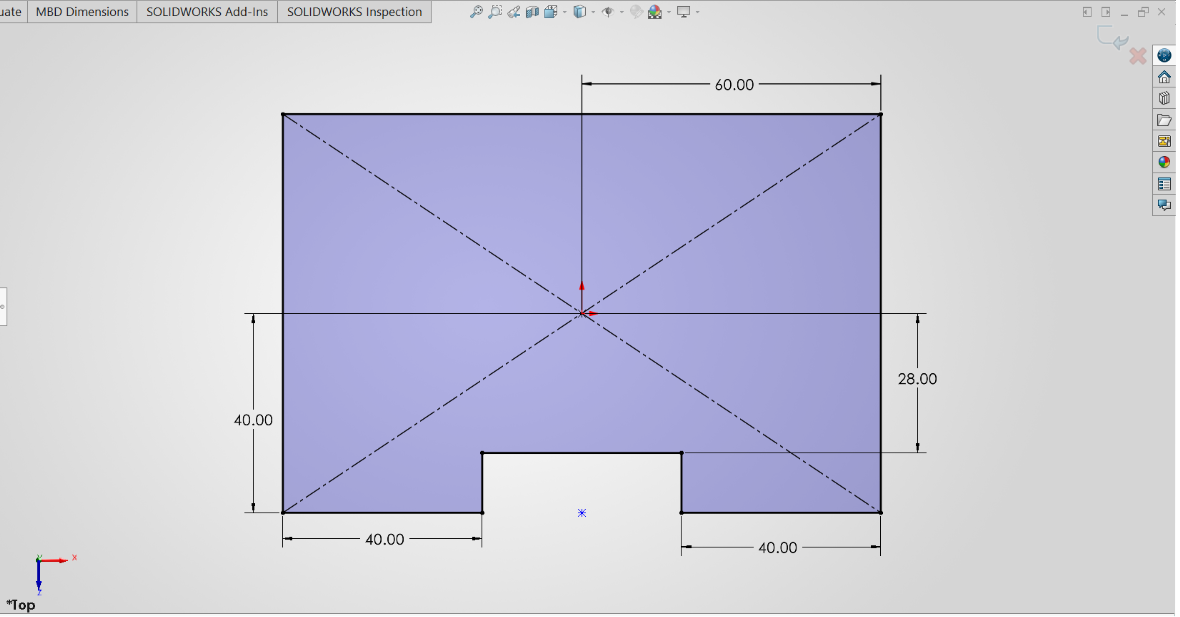
\includegraphics[width=\textwidth, keepaspectratio]{lab-01/assets/object-4/object-4-snap-1.png}
    \caption{2D sketch of the base.}
  \end{subfigure}%
  \hfill
  \begin{subfigure}[b]{0.32\textwidth}
    \centering
    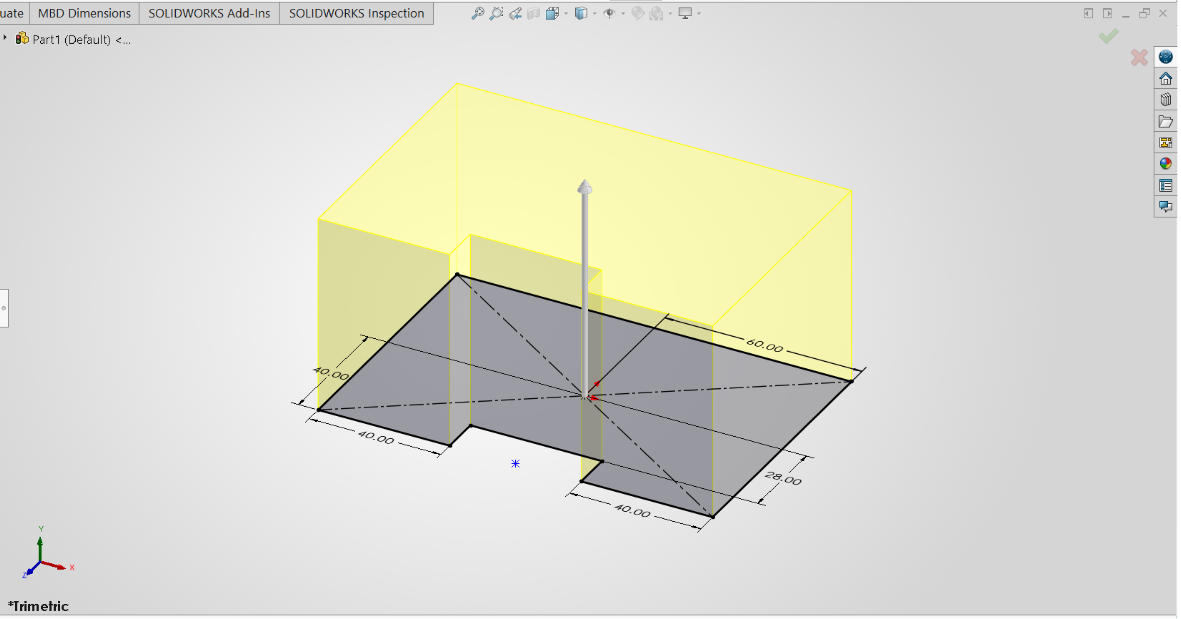
\includegraphics[width=\textwidth, keepaspectratio]{lab-01/assets/object-4/object-4-snap-2.png}
    \caption{Extruding the base sketch.}
  \end{subfigure}%
  \hfill
  \begin{subfigure}[b]{0.32\textwidth}
    \centering
    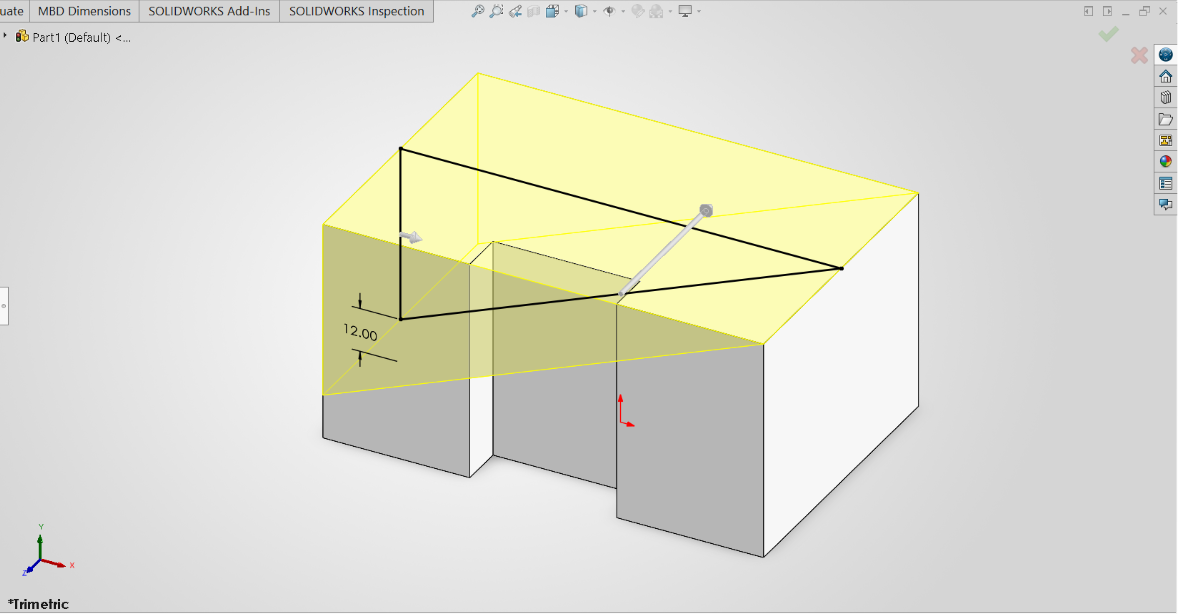
\includegraphics[width=\textwidth, keepaspectratio]{lab-01/assets/object-4/object-4-snap-5.png}
    \caption{Creating the angled cut.}
  \end{subfigure}%
  \vspace{0.5em}
  \begin{subfigure}[b]{0.49\textwidth}
    \centering
    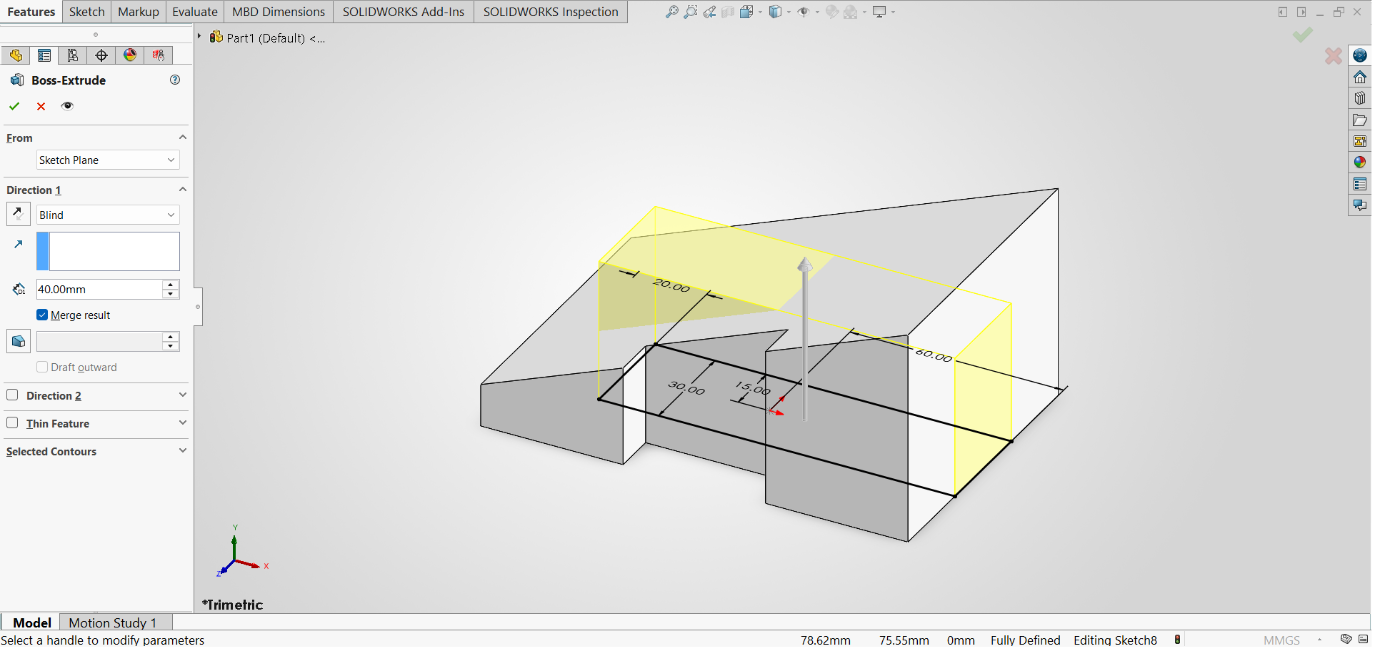
\includegraphics[width=\textwidth, keepaspectratio]{lab-01/assets/object-4/object-4-snap-8.png}
    \caption{Extruding the central block.}
  \end{subfigure}%
  \hfill
  \begin{subfigure}[b]{0.49\textwidth}
    \centering
    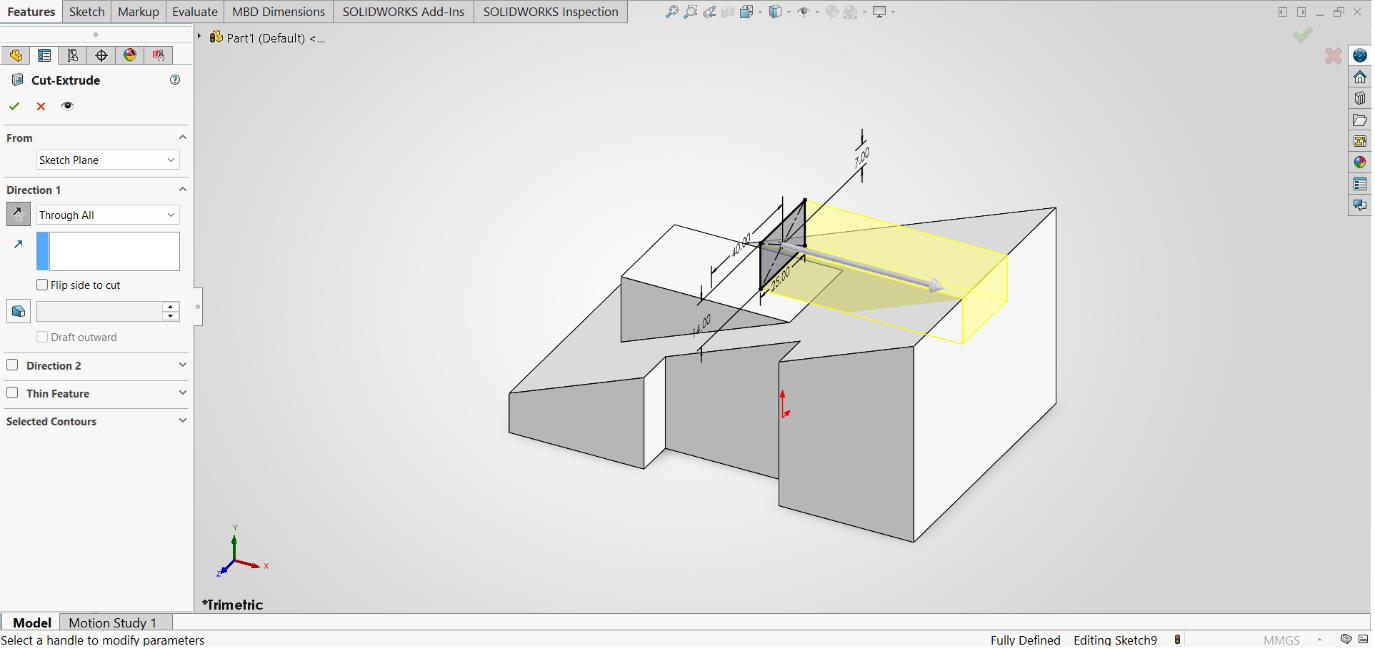
\includegraphics[width=\textwidth, keepaspectratio]{lab-01/assets/object-4/object-4-snap-11.png}
    \caption{Creating the top cut-out.}
  \end{subfigure}%
  \vspace{0.5em}
  \begin{subfigure}[b]{\textwidth}
    \centering
    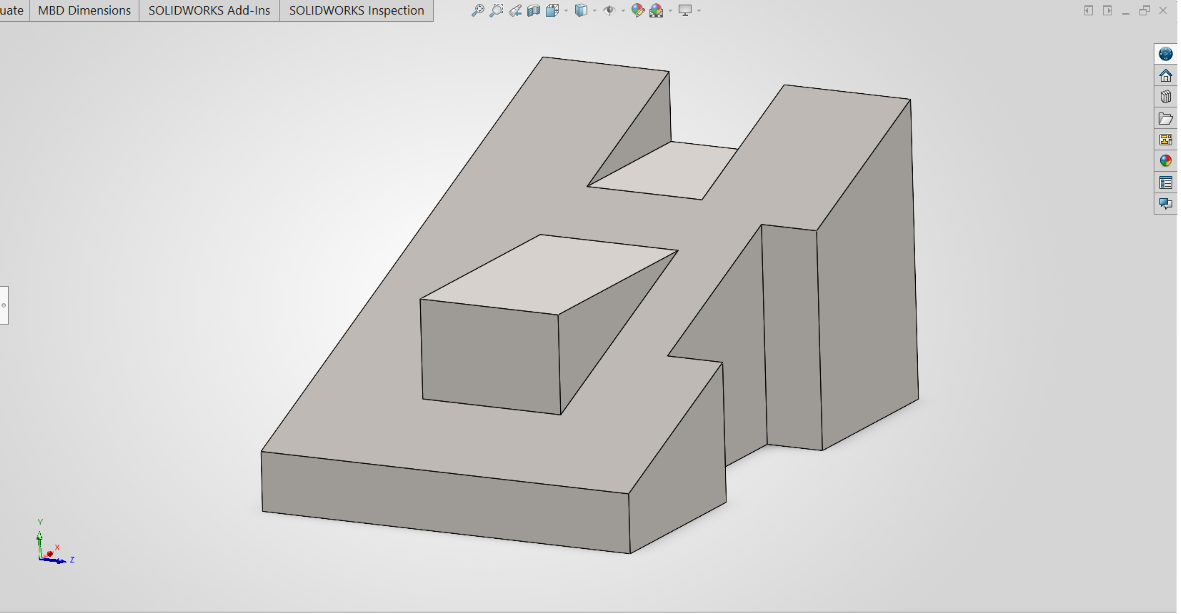
\includegraphics[width=\textwidth, keepaspectratio]{lab-01/assets/object-4/object-4-snap-12.png}
    \caption{Final result.}
  \end{subfigure}

  \caption{Snapshots while Designing Object 4 in Solidworks}
  \label{lab01_object_4}
\end{figure}
